\section{Toiminnallisen testauksen työkalujen vertailua}

Toiminnallisia testejä voi Androidilla tehdä monella eri työkalulla ja eri abstraktiotasolla. Androidin omista työkaluista toiminnallisten testien kirjoittamiseen soveltuvat AndroidInstrumentationTestCase-yliluokan avulla tehdyt JUnit-testit, Monkeyrunnerilla kirjoitetut testit sekä Uiautomator-testit. Näistä AndroidInstrumentationTestCase-luokkaa käyttävät testit ovat matalimmalla tasolla ja niiden kirjoittaminen vaatii tietoa ohjelmakoodin toiminnasta. Monkeyrunner-testit kirjoitetaan Pythonilla, eivät vaadi tietoa ohjelman sisäisestä rakenteesta, mutta koska Monkeyrunnerista puuttuvat kunnon assertointimahdollisuudet, en käsittele sitä tässä. Käsittelen sen sijaan Uiautomatorilla kirjoitettuja toiminnallisia testejä. Tämän lisäksi käsittelen Robotiumia, joka on Javalla käytettävä testityökalu sekä Troydia, joka käyttää Rubya testien tuottamiseen.

\subsection{Robotium}

Robotium on suosittu testityökalu Android-sovellusten testauksessa. Robotium pyrkii tarjoamaan Android-sovelluksille vastaavan toiminnallisuuden kuin suosittu Selenium-testikehys selaintestaukseen. Selenium on toiminnallisessa ja integraatiotestauksessa käytetty työkalu, joka mahdollistaa selaimen toimintojen automatisoimisen, kuten linkkien klikkauksen ja lomakekenttien täyttämisen koneellisesti \cite{selenium}.

Robotium on tarkoitettu Android-sovellusten toiminnalliseen, järjestelmä- ja hyväksyntätestaukseen. Se on musta laatikko -työkalu, eli testin kirjoittajan ei tarvitse päästä käsiksi tai tuntea testattavan sovelluksen koodia. Robotium-testit voivat testata samassa testitapauksessa useita aktiviteetteja. Robotium-testeissä annetaan ohjeita, missä järjestyksessä käyttöliittymäelementtejä klikataan tai syötetään tekstiä.

Robotiumtestejä voi ajaa niin emulaattorissa kuin puhelimessakin. Testit eivät kuitenkaan voi käsitellä kahta eri sovellusta, eli yksi testitapaus voi käsitellä vain yhtä sovellusta. Sovellustenvälinen integraatiotestaus ei ole mahdollista.

Robotiumin kotisivuilla sille esitellään useita vahvuuksia Android SDK:n mukana tuleviin työkaluihin verrattuna. Testit vaativat vain vähäistä tuntemusta testattavasta sovelluksesta, Robotium tukee usean aktiviteetin testaamiseta samassa testissä, testien kirjoittamisen nopeus, testikoodin selkeys ja sitkeys, joka johtuu ajoaikaisesta sidonnasta käyttöliittymäkomponentteihin, nopea suoritusnopeus ja helppo integrointi jatkuvan integroinnin työkaluihin Antin tai Mavenin avulla \cite{robotium}.

\subsection{Troyd}

Troyd on Robotiumia käyttäen tehty integraatiotestaustyökalu, jonka tavoite on yhdistää Monkeyrunnerin skriptausominaisuudet ja Robotiumin tarjoama korkean tason API. Troyd-testit käyttävät korkean tason komentoja, kuten ''paina nappia nimeltä x''  tai ''tarkista, että ruudulla näkyy teksti y'', joten testien kirjoituksen pitäisi olla nopeaa. Lisäksi Troyd tarjoaa nauhoitus-toiminnon, jolla testiä voidaan kirjoittaa siten, että testiä kirjoitettaessa ohjelma etenee aina seuraavaan tilaan testin mukaisesti. Lopuksi testi tallentuu testitapauksiksi \cite{troyd}.

Troyd-testejä kirjoitetaan Rubylla käyttäen Rubyn Test::Unit-työkalua, joka on Rubyn vakiokirjaston mukana tuleva yksikkötestityökalu \cite{testunit}. Troydin komennot sisältävä TroydCommands-moduli sisällytetään testiluokkaan käyttämällä Rubyn mixin-toiminnallisuutta. Testitapauksia voi kirjoittaa kuten tavallisia Test::Unit-testejä tai sitten voi käyttää nauhoitusmahdollisuutta.

Troydin heikkouksia on sen tekijöiden mielestä mahdollisuus testata vain yhtä sovellusta kerrallaan. Esimerkiksi, jos sovellus aukaisee selainikkunan, Troyd menettää sovelluksen kontrollin. Tämä johtuu Androidin testi-instrumentaation rajoituksista. Toinen Troydin heikkous on hidas suoritusnopeus, koska testiskripti odottaa jokaisen komennon jälkeen, että sovellus on varmasti oikeassa tilassa ennen testin jatkamista \cite{troyd}.

Troydin lähdekoodi on avoin ja se löytyy GitHubista \cite{troyd_github}.

\subsection{Aiempaa tutkimusta}

Jeon \& Foster mainitsevat Robotiumin vahvuudeksi Androidin omaa Instrumentatiota rikkaamman APIn. Esimerkiksi nappien painamiseen voidaan käyttää nappien nimeä, josta Robotium laskee napin sijainnin. He myös vertaavat Robotiumia omaan Troyd-työkaluunsa ja sanovat sen heikkoudeksi, että testit pitää määritellä etukäteen, eikä niitä pysty muokkaamaan ajonaikaisesti. Muulta toiminnallisuudeltaan Troyd ja Robotium ovat suunnilleen samankaltaisia, koska Troyd on tehty Robotiumin päälle \cite{troyd}.

Benli et al. tutkivat valkoinen laatikko ja musta laatikko -testaustapojen suhteellista tehokkuutta Android-alustalla. Musta laatikko -testeissä tutkimuksessa käytettiin Robotiumia, koska Androidin mukana tulevat testaustyökalut eivät mahdollistaneet järkevää JUnit-pohjaista musta laatikko -testausta. Valkoinen laatikko -testit tehtiin Androidin yksikkötestityökaluilla. Tuloksena oli, että valkoinen laatikko -testien kirjoittaminen kesti 89\% kauemmin, mutta testien ajaminen oli 43\% nopeampaa kuin musta laatikko -testien. Testiohjelmaan istutetut bugit löytyivät valkoinen laatikko -testeillä, mutta ei Robotium-testeillä. Testiajojen nopeuteen liittyen on huomattava, että Robotium-testit ajettiin visuaalisessa moodissa niin, että jokaisen komennon välissä oli yksi sekunti, jotta käyttöliittymän tila ehdittiin havaita manuaalisesti \cite{benli12}.

\subsection{Testiprojektista}
\label{tomdroid}

\begin{figure}[htb]
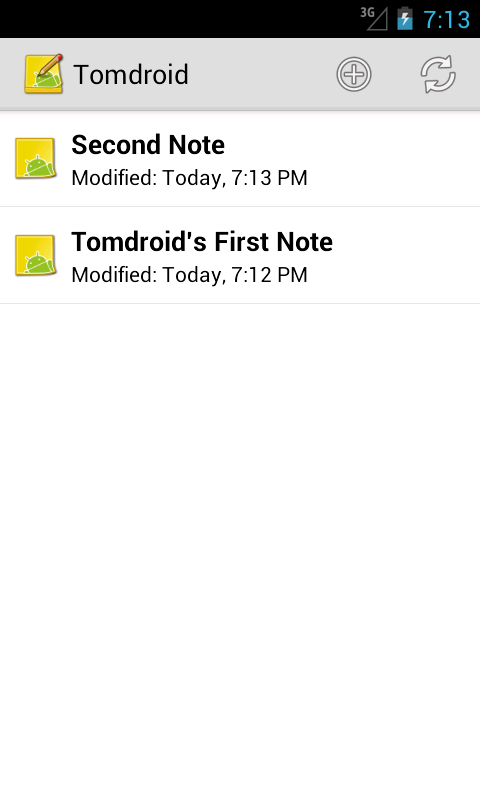
\includegraphics[width=60mm]{tomdroid_notelist.png}
\caption{Muistikirjalista Tomdroidissa} \label{tomdroid_notelist}
\end{figure}

Toiminnallisten testityökalujen vertailussa käytän testattavana ohjelmana Tomdroidia. Tomdroid on GPL-lisenssillä julkaistu avoimen lähdekoodin muistikirjasovellus \cite{tomdroid}. Tomdroid on valittu testattavaksi sovellukseksi, koska sen lähdekoodi on saatavilla, se on riittävän monimutkainen, jotta sille tehdyt testit kuvaisivat oikeassa Android-kehityksessä kohdattavia testaushaasteita, se on vasta beta-vaiheessa, joten sovelluksesta pitäisi löytyä myös bugeja ja lisäksi sovelluksen oma testaus on lähes olematonta.

Tätä tutkielmaa varten tein kopion Tomdroidin lähdekoodista versiosta 0.7.2 ja kopioin sen githubiin \cite{tomdroid_github}.

\begin{figure}[htb]
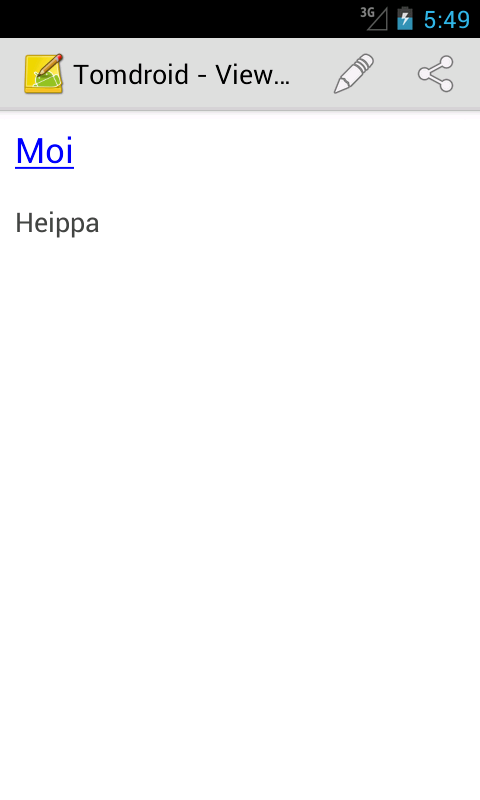
\includegraphics[width=60mm]{tomdroid_noteview.png}
\caption{Muistikirjan luku Tomdroidissa} \label{tomdroid_noteview}
\end{figure}

Tomdroidissa olennaisimmat näkymät ovat muistikirjalista, josta on ruutukaappaus kuvassa \ref{tomdroid_notelist}, yksittäisen muistikirjan selaaminen (kuvassa \ref{tomdroid_noteview}) ja sen editointi (kuvassa \ref{tomdroid_editview}). 

Listanäkymässä näkyvät kaikki käyttäjän muistikirjat päivitysajan mukaan järjestettynä. Muistikirjan koskeminen avaa kyseisen muistikirjan selausnäkymän. Yläpalkin +-symboli luo uuden muistikirjan ja avaa sen muokkausnäkymään. Yläpalkin oikeassa reunassa on synkronointi-symboli, josta muistikirjojen tila päivitetään palvelimen kanssa.

Selausnäkymässä voi lukea yksittäistä muistikirjaa. Jos tekstiä on enemmän kuin ruudulle mahtuu kerrallaan, sitä voi selata raahaamalla. Kynä-ikoni yläpalkissa avaa muistikirjan editointinäkymään. Yläpalkin oikean reunan ikonista voi jakaa muistikirjan toisiin sovelluksiin. Lisäksi vasemman yläreunan ikonista pääsee takaisin listaan.

Editointinäkymässä yläpalkissa on kuvakkeet muutosten tallentamista ja perumista varten. Tallennettaessa ruudulla näkyy hetken aikaa leijuke, jossa kerrotaan muutosten tallennuksesta. Painettaessa peru-nappia ruudulle tulee dialogi, jossa pitää vahvistaa peruminen edelliseen tallennettuun versioon. Lisäksi vasemman yläreunan ikonista pääsee takaisin listaan.

\begin{figure}[htb]
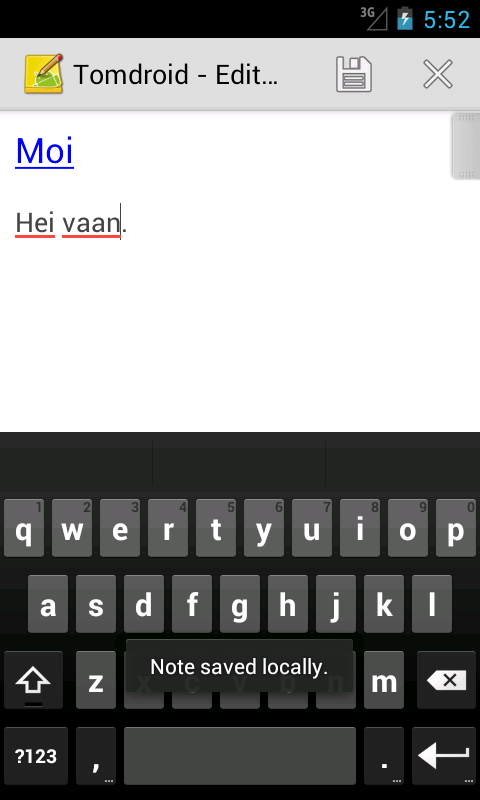
\includegraphics[width=60mm]{tomdroid_editview.png}
\caption{Muistikirjan editointi Tomdroidissa} \label{tomdroid_editview}
\end{figure}

\subsection{Testitapaus}

Testaan samaa testitapausta jokaisella työkalulla. Testitapauksessa luodaan uusi muistikirja, jonka otsikoksi kirjoitetaan ''new note'' ja tallennetaan se.

Ensimmäisenä sovellus käynnistetään ja varmistetaan, ettei muistikirjalistassa ole vielä ''new note''-nimistä muistikirjaa. Tämän jälkeen painetaan yläpalkin +-symbolia, josta päästään uuden muistikirjan muokkausnäkymään. Muokkausnäkymässä valitaan otsikon muokkaus -kenttä ja kirjoitetaan siihen ''new note''. Sitten muistikirja tallennetaan painamalla yläpalkin tallennus-symbolia. Tallentamisen jälkeen palataan listanäkymään painamalla yläpalkin vasemman reunan ikonista. Listanäkymässä varmistetaan, että muistikirja on tallentunut katsomalla, että listasta löytyy nyt ''new note''-niminen muistikirja.

Testitapaus testaa Tomdroidin perustoiminnallisuudet: muistikirjan luonnin, muokkauksen, tallennuksen ja listanäkymän. Testitapauksen toteuttaminen vaatii, että testityökalussa on perustoiminnallisuudet: elementtejä voi etsiä tekstin perusteella, erilaisia ikoneita eri puolilla näyttöä voi painaa ja tekstikenttiin voi syöttää tekstiä.

\subsection{Asennukset}

\begin{lstlisting}[float,label=robotium_setup,caption=Robotium-testirunko]
public class RobotiumTest extends ActivityInstrumentationTestCase2<Tomdroid> {

	private Solo solo;
	
	public RobotiumTest() {
		super(Tomdroid.class);
	}
	
	@Override
	public void setUp() {
		solo = new Solo(getInstrumentation(), getActivity());
	}
	
	@Override
	public void tearDown() throws Exception {
		solo.finishOpenedActivities();
	}
}
\end{lstlisting}

Robotiumin asennus on yksinkertaista. Projektin build pathiin tarvitsee vain lisätä Robotiumin jar-paketti, jossa tulee kaikki tarvittava mukana. Itse Robotium-testit perivät Androidin omasta ActivityInstrumentationTestCase2-yliluokasta. Listauksessa \ref{robotium_setup} on esitetty Robotium-testin runko ilman varsinaisia testejä. setUp()-metodissa alustetaan Solo, joka on Robotiumin testit suorittava olio. Se ottaa konstruktoriparametreina ActivityInstrumentationTestCase2:n tarjoaman instrumentaation ja testattavan aktiviteetin. tearDown()-metodissa kutsutaan finishOpenedActivities()-metodia, joka lopettaa kaikki testin aikana aktiivisena olleet aktiviteetit.

\begin{lstlisting}[float,label=delete_notes,caption=Muistikirjojen poisto]
private void removeAllNotes() {
	NoteManager.deleteAllNotes(getActivity());
}
\end{lstlisting}

Robotium-testeissä on huomattava, että jos sovellus muuttaa muistikortille tai muualle tallennettua tilaansa, on testeissä manuaalisesti pidettävä huolta, että sovellus resetoidaan takaisin alkuperäiseen tilaan, jotta testejä voi toistaa useita kertoja luotettavasti. Tomdroidin tapauksessa tämä tehtäisiin kutsumalla tearDown():ssa apumetodia removeAllNotes(), joka on esitetty listauksessa \ref{delete_notes}. Metodi kutsuu Tomdroidin NoteManagerin deleteAllNotes()-metodia, joka poistaa kaikki sovelluksen tallentamat muistikirjat.

\begin{lstlisting}[float, label=troyd_run, caption=Troyd-nauhoitusskriptin ja testien ajaminen]
ruby bin/rec.rb apks/org.tomdroid.apk
ruby bin/trun.rb
\end{lstlisting}

Troyd vaatii toimiakseen Rubyn version 1.8.7 sekä nokogiri-xml-kirjaston. Lisäksi se tukee vain Androidin versiota 2.3.6, joten uudemman Android-version vaativien sovellusten testaaminen ei ole sillä mahdollista. Troydin asennus kesti huomattavasti Robotiumin asennusta kauemmin, vaikka koneellani oli valmiiksi asennettuna Rubyn versionhallintatyökalu rvm \cite{rvm}, jolla oikean ruby-version asennus onnistuu yhdellä komennolla. Rubyn versio 1.8.7 on julkaistu kesällä 2008 ja sen päivitykset loppuivat kesäkuussa 2013 \cite{ruby_187}, joten joissain järjestelmissä näin vanhan version asennus voi olla haasteellista. Asennusten jälkeen Troydin testin kirjoittaminen onnistui kuitenkin nopeasti nauhoitusskriptin avulla, joka hoiti kaiken muun kuin itse testikoodin kirjoittamisen. Nauhoitus ja ajoskriptit on esitetty listauksessa \ref{troyd_run}. rec.rb on nauhoitusskripti, jolla testit kirjoitetaan ja run.rb ajoskripti, joka ajaa oletuksena kaikki testcases-hakemistosta löytyvät testit. Testit voivat olla myös eri sovelluksille, jolloin Troyd asentaa kunkin testattavan sovelluksen erikseen.

\begin{lstlisting}[float, label=uiautomator_run,caption=Uiautomator-testien ajaminen]
#!/bin/sh
ant build
adb push bin/TomdroidUiAutomatorTest.jar /data/local/tmp/
adb shell uiautomator runtest TomdroidUiAutomatorTest.jar -c org.tomdroid.test.UiAutomatorTest
\end{lstlisting}

Uiautomator vaatii vähintään Androidin API-version 16, jonka mukana tulee uiautomator.jar-paketti, joka täytyy asettaa testiprojektin riippuvuuksiin Androidin ja JUnitin ohella. Lisäksi testien ajaminen vaatii tietokoneessa kiinni olevan Android-laitteen, johon testattava sovellus on asennettuna. Testien kääntäminen ja ajaminen on esitetty listauksessa \ref{uiautomator_run}. Testit käännetään Apache Antilla \cite{ant}, joka on avoimen lähdekoodin käännöstyökalu Java-sovelluksille. Toisella rivillä käytetään Androidin mukana tulevaa adb-työkalua (\emph{Android debug bridge}) käännetyn testisovelluksen siirtämiseen puhelimeen ja kolmannella rivillä ajetaan testisovelluksesta luokka org.tomdroid.test.UiAutomatorTest.

\subsection{Robotium-testit}

\begin{lstlisting}[float,label=robotium_createnote,caption=Muistikirjan luontitesti Robotiumilla]
public void testCreateNoteAddsNote() {
	solo.assertCurrentActivity("Testi alkoi väärästä aktiviteetista", Tomdroid.class);
	assertFalse(solo.searchText("new note"));
	solo.clickOnActionBarItem(R.id.menuNew);
	solo.assertCurrentActivity("Uuden muistikirjan luonti ei avannut editointinäkymää", EditNote.class);
	solo.enterText(0, "new note");
	solo.clickOnActionBarItem(R.id.edit_note_save);
	solo.clickOnActionBarHomeButton();
	solo.assertCurrentActivity("Koti-näppäimen painaminen ei vienyt takaisin muistikirjalistaan", Tomdroid.class);
	assertTrue(solo.searchText("new note"));
}
\end{lstlisting}

Robotium-testi, jossa testataan uuden muistikirjan luonti, on esitetty listauksessa \ref{robotium_createnote}. Robotiumilla testiä ohjataan Solo-luokan instanssin kautta, jossa on sovelluksen kanssa kommunikointiin tarkoitettuja metodeja, sovelluksen tilasta kertovia metodeja sekä assertteja. Testin ensimmäisellä rivillä käytetään assertCurrentActivity()-metodia asserttia varmistamaan, että testi alkaa muistikirjalistasta. Toisella rivillä varmistetaan, että testissä luotavaa muistikirjaa ei vielä löydy listasta. Seuraavalla rivillä painetaan yläpalkin uuden muistikirjan luovaa nappia clickOnActionBarItem()-metodilla. Se ottaa parametrina id:n siitä komponentista, johon ollaan painamassa. Tämän jälkeen pitäisi avautua uusi muistikirja editointinäkymään, mikä varmistetaan seuraavalla rivillä. Sitten syötetään enterText()-metodilla uuden muistikirjan otsikoksi ''new note''. Ensimmäinen parametri kertoo, monenteenko ruudulla näkyvään tekstinmuokkauskomponenttiin teksti syötetään. Tämän jälkeen klikataan yläpalkin tallennus-nappia ja sitten muistikirjalistaukseen vievää nappia. Lopuksi vielä varmistetaan, että palattiin takaisin muistikirjalistaan ja listasta löytyy nyt juuri luotu aktiviteetti.

\subsection{Troyd-testit}

\begin{lstlisting}[float, label=troyd_createnote,caption=Muistikirjan luontitesti Troydilla]
def test_"create note adds note"
  click "OK"
  assert_not_text "new note"
  clickImg 1
  edit 0, "new note"
  clickImg 1
  clickImg 0
  assert_text "new note"
end
\end{lstlisting}

Troyd-testi, jossa luodaan muistikirja, on esitetty listauksessa \ref{troyd_createnote}. Troyd-testit asentavat aina ensimmäisenä uuteen emulaattoriin koko sovelluksen, joten Robotium-testissä tarvittuja vanhojen muistikirjojen poistoa ei tarvita. Tein testin Troydin nauhoitusskriptin avulla, joten itse testi on automaattisesti kirjoitettu tämän pohjalta. Testitiedosto sisältää testimetodin lisäksi metodit sovelluksen alustamiselle ja lopettamiselle sekä testeissä käytetyt Ruby-metodit, mutta nämä kaikki Troyd tuotti automaattisesti nauhoitusskriptin avulla. Itse testimetodin sisältö on sama kuin testiskriptissä kirjoittamani komennot. Lisäksi näin sovelluksen testiä vastaavassa tilassa emulaattorissa testiä kirjoittaessa, mikä helpotti testin kirjoittamista. Listauksesta on lisäksi huomattava, että Rubyssa metodien sulut ovat vapaaehtoiset, mikäli sekaantumisen vaaraa ei ole. Siksi testissä metodien parametrit eivät ole sulkujen sisällä. Kun nauhoitusskriptissä on saanut haluamansa testitapauksen valmiiksi, se tallennetaan sofar-metodilla, jonka parametrina on testin nimi, kuten on tehty listauksessa \ref{troyd_record_save}. Finish-komento lopettaa nauhoitusskriptin.

\begin{lstlisting}[float, label=troyd_record_save,caption=Testin tallennus nauhoitusskriptistä Troydilla]
sofar "create note adds note"
finish
\end{lstlisting}

Testin ensimmäisellä rivillä painetaan OK-nappia, koska sovellus näyttää ensimmäisellä käynnistyskerralla ohje-tekstin. Troydilla ei voi varmistaa, missä aktiviteetissa ollaan, kuten Robotium-testissä tehtiin, joskin listan tähän mennessä vierailluista aktiviteeteista saisi getActivities-metodilla. Troyd ei myöskään tue Robotium-testissä käytettyä R-luokan id:n perusteella elementtien etsimistä, vaan elementit etsitään indeksin perusteella järjestyksessä ruudulta. Sen takia testi luettuna ei ole yhtä selkeä, kuin Robotium-testit. Tässä testissä ensimmäinen clickImg-metodi painaa uuden muistikirjan luovaa nappia, toinen clickImg tallennus-nappia ja kolmas clickImg palaa takaisin listaukseen -nappia.

Testien kirjoittaminen sujui Troydilla nopeasti, mutta toisaalta osaan Rubya yhtä hyvin kuin Javaakin, joten erilainen syntaksi ei häirinnyt kirjoitusta. Nauhoitusskripti on kuitenkin vielä hieman raakile, esimerkiksi ruudulta löytymättömän indeksin klikkaaminen kaatoi sovelluksen ja pakotti aloittamaan nauhoituksen alusta.

\subsection{Uiautomator-testit}

\begin{lstlisting}[float, label=uiautomator_createnote,caption=Muistikirjan luontitesti Uiautomatorilla]
public class UiAutomatorTest extends UiAutomatorTestCase {
  public void testCreateNoteAddsNote() throws UiObjectNotFoundException {
    getUiDevice().pressHome();
    UiSelector selector = new UiSelector().text("Tomdroid")
    UiObject targetApp = new UiObject(selector);
    targetApp.clickAndWaitForNewWindow();
    selector = new UiSelector().text("new note")
    UiObject newNoteText = new UiObject(selector);
    assertFalse(newNoteText.exists());
    selector = new UiSelector().description("New")
    UiObject newNoteButton = new UiObject(selector);
    newNoteButton.clickAndWaitForNewWindow();
    selector = new UiSelector().className("android.widget.EditText")
    UiObject titleEditText = new UiObject(selector);
    titleEditText.setText("new note");
    selector = new UiSelector().description("Save")
    UiObject saveButton = new UiObject(selector);
    saveButton.click();
    selector = new UiSelector().description("Siirry etusivulle")
    UiObject homeButton = new UiObject(selector);
    homeButton.clickAndWaitForNewWindow();
    selector = new UiSelector().text("new note")
    newNoteText = new UiObject(selector);
    assertTrue(newNoteText.exists());  
    removeCreatedNote(newNoteText);
  }
}
\end{lstlisting}

Listauksessa \ref{uiautomator_createnote} on esitetty Uiautomator -testi, jossa luodaan uusi muistikirja. Testi perii yliluokan UiAutomatorTestCase. Testeissä ajetaan JUnit3-tyylin mukaisesti test-alkuiset metodit. Testimetodi heittää UiObjectNotFoundExceptionin, jos yritetään tehdä interaktiota komponentin kanssa, jota ei lyödetty selectorilla. Testissä käytetään pääosin kahta UiAutomatorin mekaniikkaa. UiSelectorin eri metodeilla etsitään käyttöliittymäelementtejä, joiden avulla konstruoidaan UiObject-olioita, joiden kanssa sitten kommunikoidaan tai kysytään niiden tilaa. 

Testissä käytetään kolmea eri UiSelectorin hakumetodia: text()-metodi hakee käyttöliittymäelementtiä, johon liittyy parametrina annettu näkyvä teksti, description()-metodi käyttää hakemiseen elementille liitettyä selitettä, esimerkiksi resurssi-tiedoston kautta annettua. className()-metodi etsii kaikki elementit, jotka ovat annetun luokan ilmentymiä, ja palauttaa niistä ensimmäisen.

UiObjectin metodeista testeissä käytetään seuraavia: clickAndWaitForNewWindow() painaa käyttöliittymäelenettiä ja odottaa seuraavan aktiviteetin latautumista, exists() palauttaa true, jos elementti löytyy ruudulta, setText()-kirjoittaa elementtiin parametrina annetun tekstin. click()-metodi painaa elementtiä, mutta ei jää odottamaan uutta aktiviteettia.

Ui automator -testit alkavat siitä tilasta, missä puhelin on testin käynnistyessä, joten on hyvä tapa aloittaa kaikki testit painamalla kotinäppäintä, jolla puhelin palautuu aloitusruutuun. Testissä oletin, että Tomdroid löytyy aloitusnäytöltä, joten seuraavaksi testissä etsitään ruudulta elementtiä, johon liittyy Tomdroid-teksti, eli sovelluksen käynnistysikoni. Yleisempi ratkaisu olisi avata lista kaikista sovelluksista ja etsiä testisovellus sitä kautta.

Kun sovellus on avattu, testi etenee kuten Robotium-testissäkin. Ensin varmistetaan, että ''new note''-nimistä muistikirjaa ei löydy valmiiksi listalta, sitten painetaan uusi muistikirja -nappia. Seuraavaksi etsitään ensimmäinen EditText-elementti ruudulta, ja syötetään siihen muistikirjan nimi. Sitten tallennetaan muistikirja, palataan muistikirjalistaan ja varmistetaan, että muistikirja tallentui.

\begin{lstlisting}[float,label=uiautomator_teardown,caption=Luodun muistikirjan poisto Uiautomatorilla] 
private void removeCreatedNote(UiObject noteText) throws UiObjectNotFoundException {
  noteText.clickAndWaitForNewWindow();
  UiSelector selector = new UiSelector().description("Lisää asetuksia")
  UiObject moreOptionsButton = new UiObject(selector);
  moreOptionsButton.click();
  selector = new UiSelector().text("Delete")
  UiObject deleteButton = new UiObject(selector);
  deleteButton.click();
  selector = new UiSelector().text("Yes")
  UiObject confirmButton = new UiObject(selector);
  confirmButton.clickAndWaitForNewWindow();
}
\end{lstlisting}

Lopuksi testissä kutsutaan removeCreatedNote()-metodia, joka on esitetty listauksessa \ref{uiautomator_teardown}. Metodi poistaa juuri luodun muistikirjan. Koska Uiautomator-testit eivät pääse käsiksi ohjelmakoodiin kuten Robotium-testit, joudutaan tehdyt muutokset perumaan käyttöliittymän kautta. Poistometodi saa parametrinaan valmiiksi viitteen luotuun muistikirjaan etusivulla, joten, sitä ei tarvitse hakea uudestaan.

\subsection{Testien suoritusnopeudet}

\begin{table}[h]
\centering
\begin{tabular}{ l l l l }
   & Keskiarvo (s) & Max (s) & Min (s) \\
  Robotium & 14,207 & 14,303 & 14,147 \\
  Troyd & 143,778 & 145,961 & 142,304 \\
  UI Automator & 16,186 & 16,506 & 15,883 \\
\end{tabular}
\caption{Testikestot}
\label{uitest_timing}
\end{table}

Eri testityökalujen testien ajoajat on esitetty taulukossa \ref{uitest_timing}. Ajoin kaikilla työkaluilla testisarjan viidesti ja mittasin testiaikojen keskiarvon ja hitaimman ja nopeimman testiajon. Testiajoon sisältyy vain muistikirjan luontitesti kerran ajettuna. 

Robotium-testit ajoin Eclipsestä Android JUnitilla emulaattorissa. Ajat ovat Eclipsen ottamia. Emulaattori oli valmiiksi käynnissä testejä ajettaessa. Testiajoon sisältyy siis sovelluksen asennus emulaattoriin ja testin ajaminen.

Troyd-testit ajoin emulaattorissa trun.rb-skriptillä ja ajastin unixin time-työkalulla. Testiajoa hidastaa se, että joka ajokerralla emulaattori käynnistetään ja testattava sovellus asennetaan emulaattoriin. Toisaalta tästä syystä testien kirjoittaminen on helpompaa, koska sovellusta ei tarvitse palauttaa testejä edeltävään tilaan kuten Robotiumilla ja Uiautomatorilla ajaessa.

Uiautomator-testit ajoin listauksessa \ref{uiautomator_run} esitetyllä shell-skriptillä Samsungin Galaxy Nexus -puhelimessa ja ajoitin testit unixin time-työkalulla. Testiajon kestoon sisältyy testien kääntäminen, siirtäminen puhelimeen ja itse testiajo. Uiautomator-testin kestoon sisältyy myös luodun muistikirjan poisto käyttöliittymästä. Testeissä oletetaan, että sovellus on valmiiksi asennettuna koneeseen kytkettyyn puhelimeen.

Troyd-testit osoittautuivat selvästi hitaammaksi kuin Robotium ja UIautomator. Robotium-testit olivat hieman UIautomator -testejä nopeammiksi, mutta ero ei ole kovin merkittävä.

\subsection{Analyysi}

Perusominaisuuksien testaus onnistui niin Troydilla, Robotiumilla kuin UI Automatorillakin.

Troydilla testaus on korkeimmalla abstraktiotasolla testatuista työkaluista. Ohjelman tilan seuraaminen testiä nauhoitettaessa nopeuttaa ja helpottaa testien kirjoitusta. Rubylle tehty API on ilmaisuvoimainen. Troyd on kuitenkin selvästi vielä kehittymätön. Se tukee vain vanhaa Android- ja Ruby-versiota ja testien suoritus on kymmenen kertaa hitaampaa kuin muilla testatuilla kehyksillä - joskin testien suoritusnopeus ei toiminnallisessa testauksessa ole yhtä kriittistä kuin yksikkötestauksessa. Lisäksi Troyd vaatii erillisen ohjelmointiympäristön normaaliin Android-kehitykseen verrattuna, eivätkä kaikki Android-kehittäjät osaa Rubya.

Robotiumilla kirjoitetut testit ovat myös melko ilmaisuvoimaisia ja tiiviitä. Robotiumin APIn oppii helposti ja testejä tehdään samoilla työkaluilla kuin muutakin Android-kehitystä. Robotium myös tukee kaikkia Androidin versioita. Robotiumin käyttö vaatii kuitenkin hieman enemmän tietoa testattavasta sovelluksesta. Suoritusnopeudeltaan Robotium-testit olivat testatuista testikehyksistä nopeimmat.

Uiautomatorin erikoisuus on siihen liittyvä Uiautomatorviewer, jonka avulla testattavan sovelluksen käyttöliittymäelementit on helppo analysoida ilman sovelluksen lähdekoodia. Työkalu nopeuttaa testien kirjoittamista huomattavasti. Tietoja voisi myös käyttää Robotium-testien kirjoittamisessa. Itse Uiautomator-testit ovat hieman verboosimpia kuin Robotium-testit, mutta niiden kirjoittaminen on hyvin suoraviivaista. Uiautomatorin suurin puute on, että se toimii vain uusimmissa Android-versioissa, joten regressiotestaus vanhempien laitteiden toiminnan varmistamiseksi ei ole mahdollista.

Työkaluista ainoastaan Robotium toimii ilman varauksia erilaisissa Android-ympäristöissä ja on siten vahvin valinta toiminnallisen testauksen työkaluksi. Uiautomator on mielenkiintoinen, mutta sen toiminta vain uusimmissa Android-versioissa rajoittaa toistaiseksi sen käyttökelpoisuutta. Troyd taas vaatii kehitystä tullakseen varteenotettavaksi vaihtoehdoksi.